\subsection{Home}
Upon launching the application, the user is greeted by a tabbed interface that divides the app into two primary sections: the Installed Widgets page and the Slideshows page. A floating action button located at the center of the bottom navigation bar changes its function depending on the active tab. When viewing the Installed Widgets page, the button displays a shopping bag icon, which opens the widget store when clicked. On the Slideshows page, the button instead shows a "plus" icon, which initiates the creation of a new slideshow.

\begin{figure}[h]
    \centering
    \begin{minipage}[b]{0.45\textwidth}
        \centering
        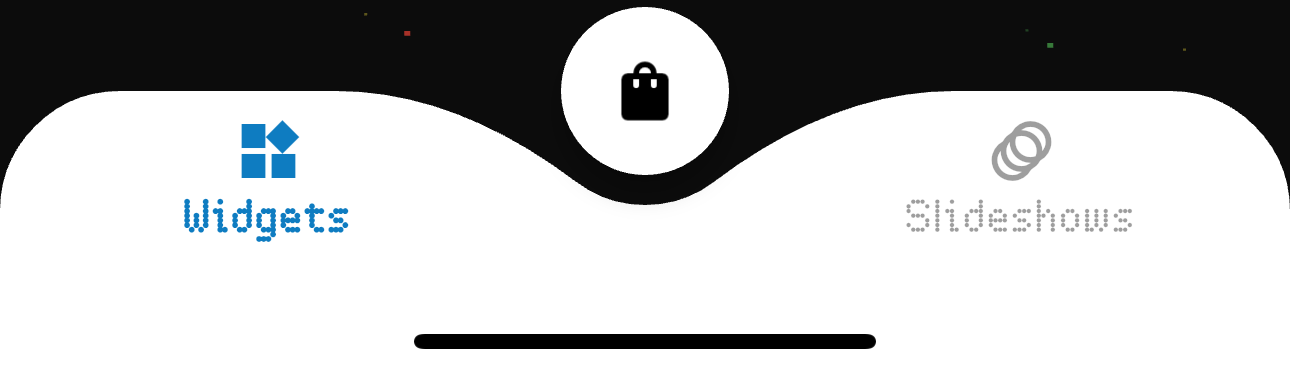
\includegraphics[width=\textwidth]{tesi/img/tab_bar/tab-bar-widgets.png}
        \caption*{Widgets Tab}
    \end{minipage}
    \begin{minipage}[b]{0.45\textwidth}
        \centering
        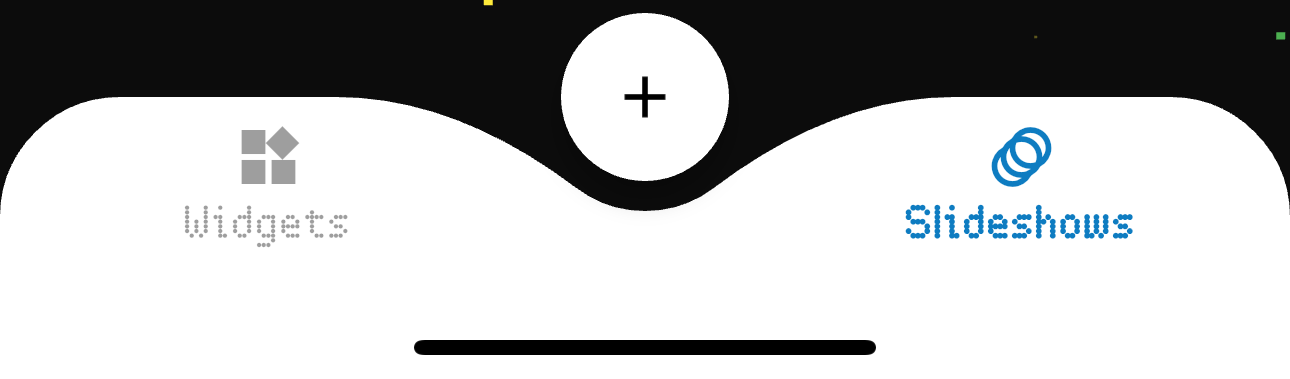
\includegraphics[width=\textwidth]{tesi/img/tab_bar/tab-bar-slideshows.png}
        \caption*{Slideshows Tab}
    \end{minipage}
\end{figure}

\subsection{Matrix Control}
At the top of the screen, a sliding panel displays essential information such as the connection status and the currently active widget. Pulling the panel down reveals further details about the matrix connection, including additional configuration options. Users can perform actions such as stopping playback or manually inputting the matrix's address.

\begin{figure}[h]
    \centering
    \begin{minipage}[b]{0.32\textwidth}
        \centering
        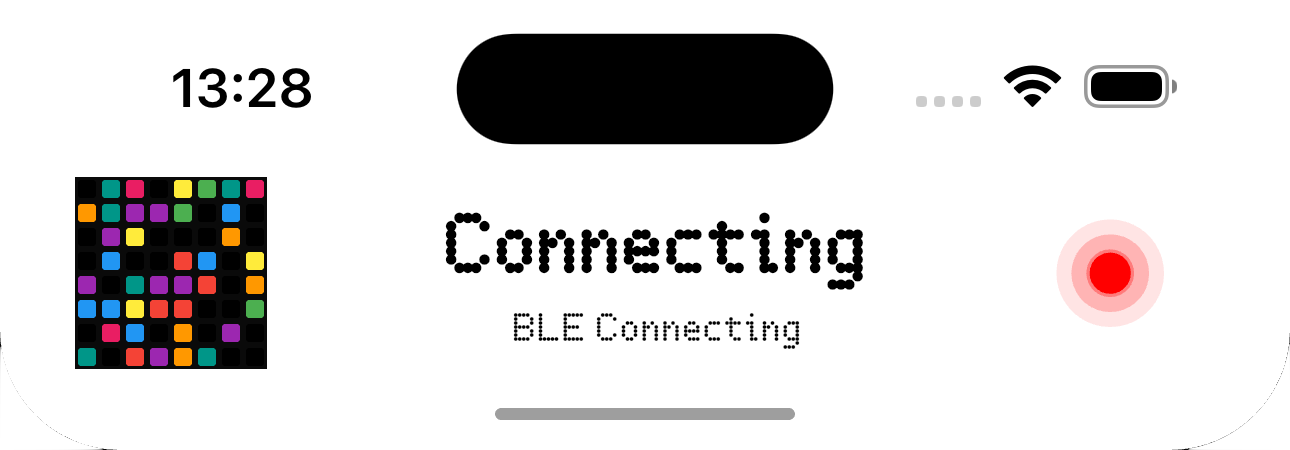
\includegraphics[width=\textwidth]{tesi/img/matrix_status_notch/connecting.png}
        \caption*{Connecting to Matrix}
    \end{minipage}
    \begin{minipage}[b]{0.32\textwidth}
        \centering
        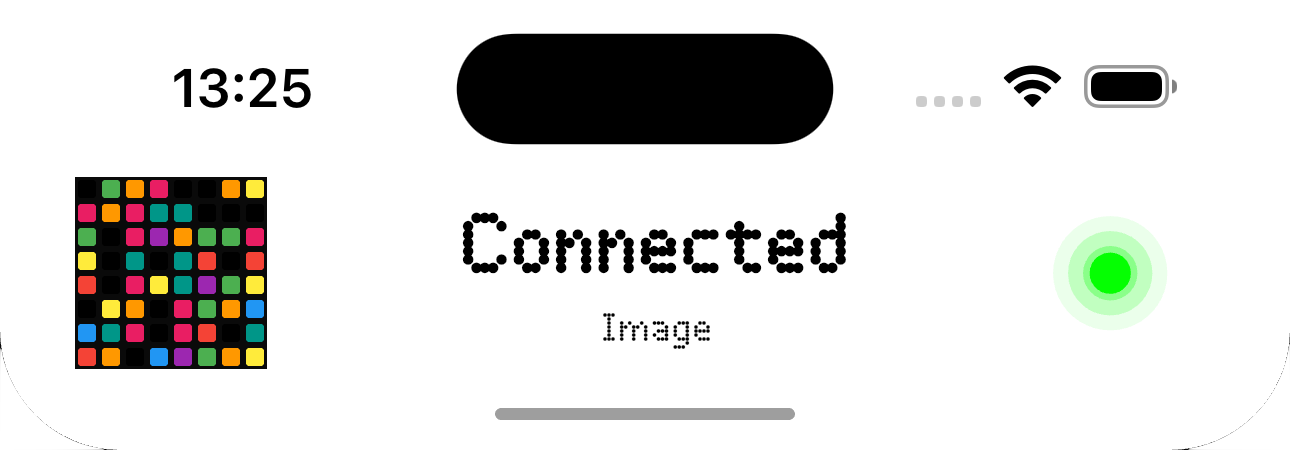
\includegraphics[width=\textwidth]{tesi/img/matrix_status_notch/connected.png}
        \caption*{Matrix Connected}
    \end{minipage}
    \begin{minipage}[b]{0.32\textwidth}
        \centering
        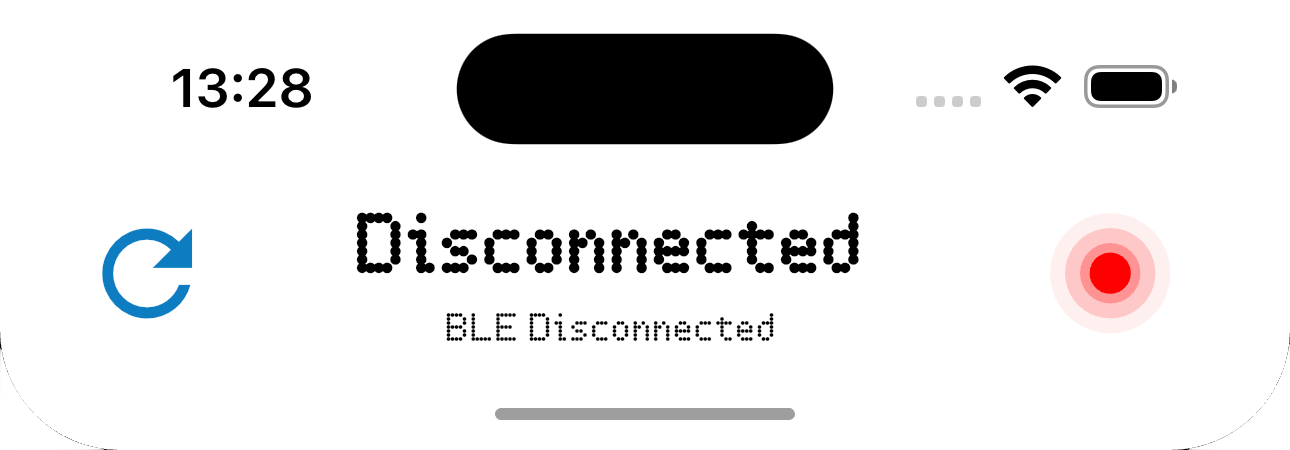
\includegraphics[width=\textwidth]{tesi/img/matrix_status_notch/disconnected.png}
        \caption*{Matrix Not Reachable}
    \end{minipage}
\end{figure}

\newpage

\subsection{Installed Widgets}
This is the default screen presented when the app launches. It lists all the widgets currently installed on the matrix, which have been downloaded from the store. Users can activate a widget by simply tapping on it. If the widget does not require further configuration, it will be displayed immediately on the matrix. However, if it is configurable, a configuration selector will prompt the user to choose a specific configuration before activating the widget.

\begin{figure}[h]
    \centering
    \begin{minipage}[b]{0.32\textwidth}
        \centering
        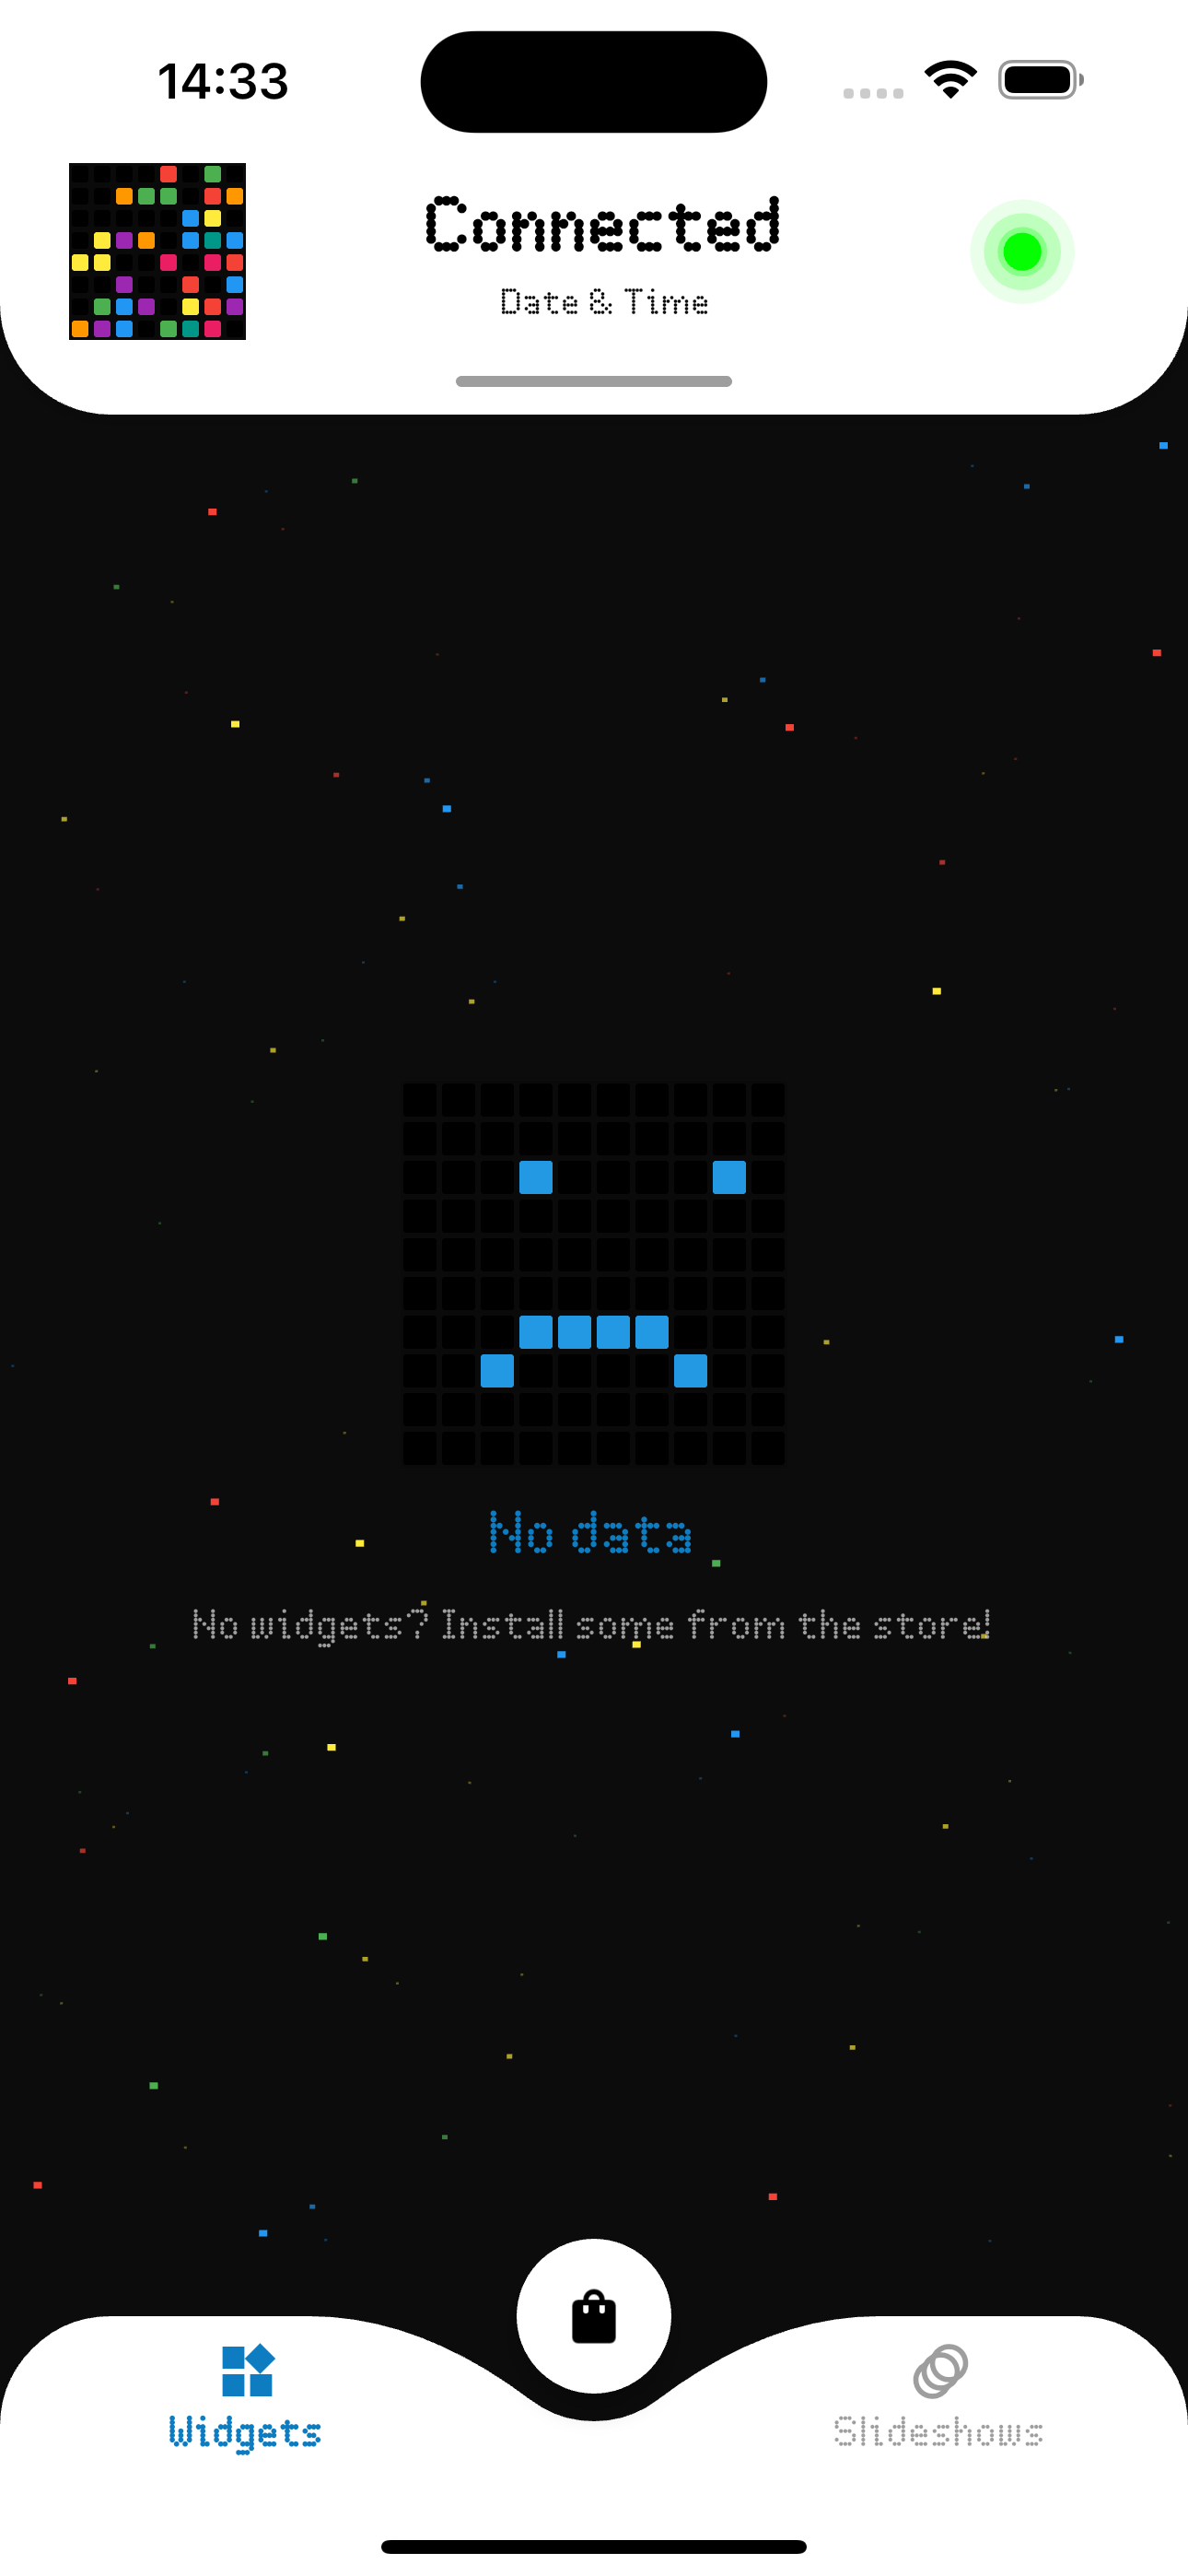
\includegraphics[width=\textwidth]{tesi/img/client_demo/installed_widgets/no_data.png}
        \caption*{No Widgets Installed}
    \end{minipage}
    \begin{minipage}[b]{0.32\textwidth}
        \centering
        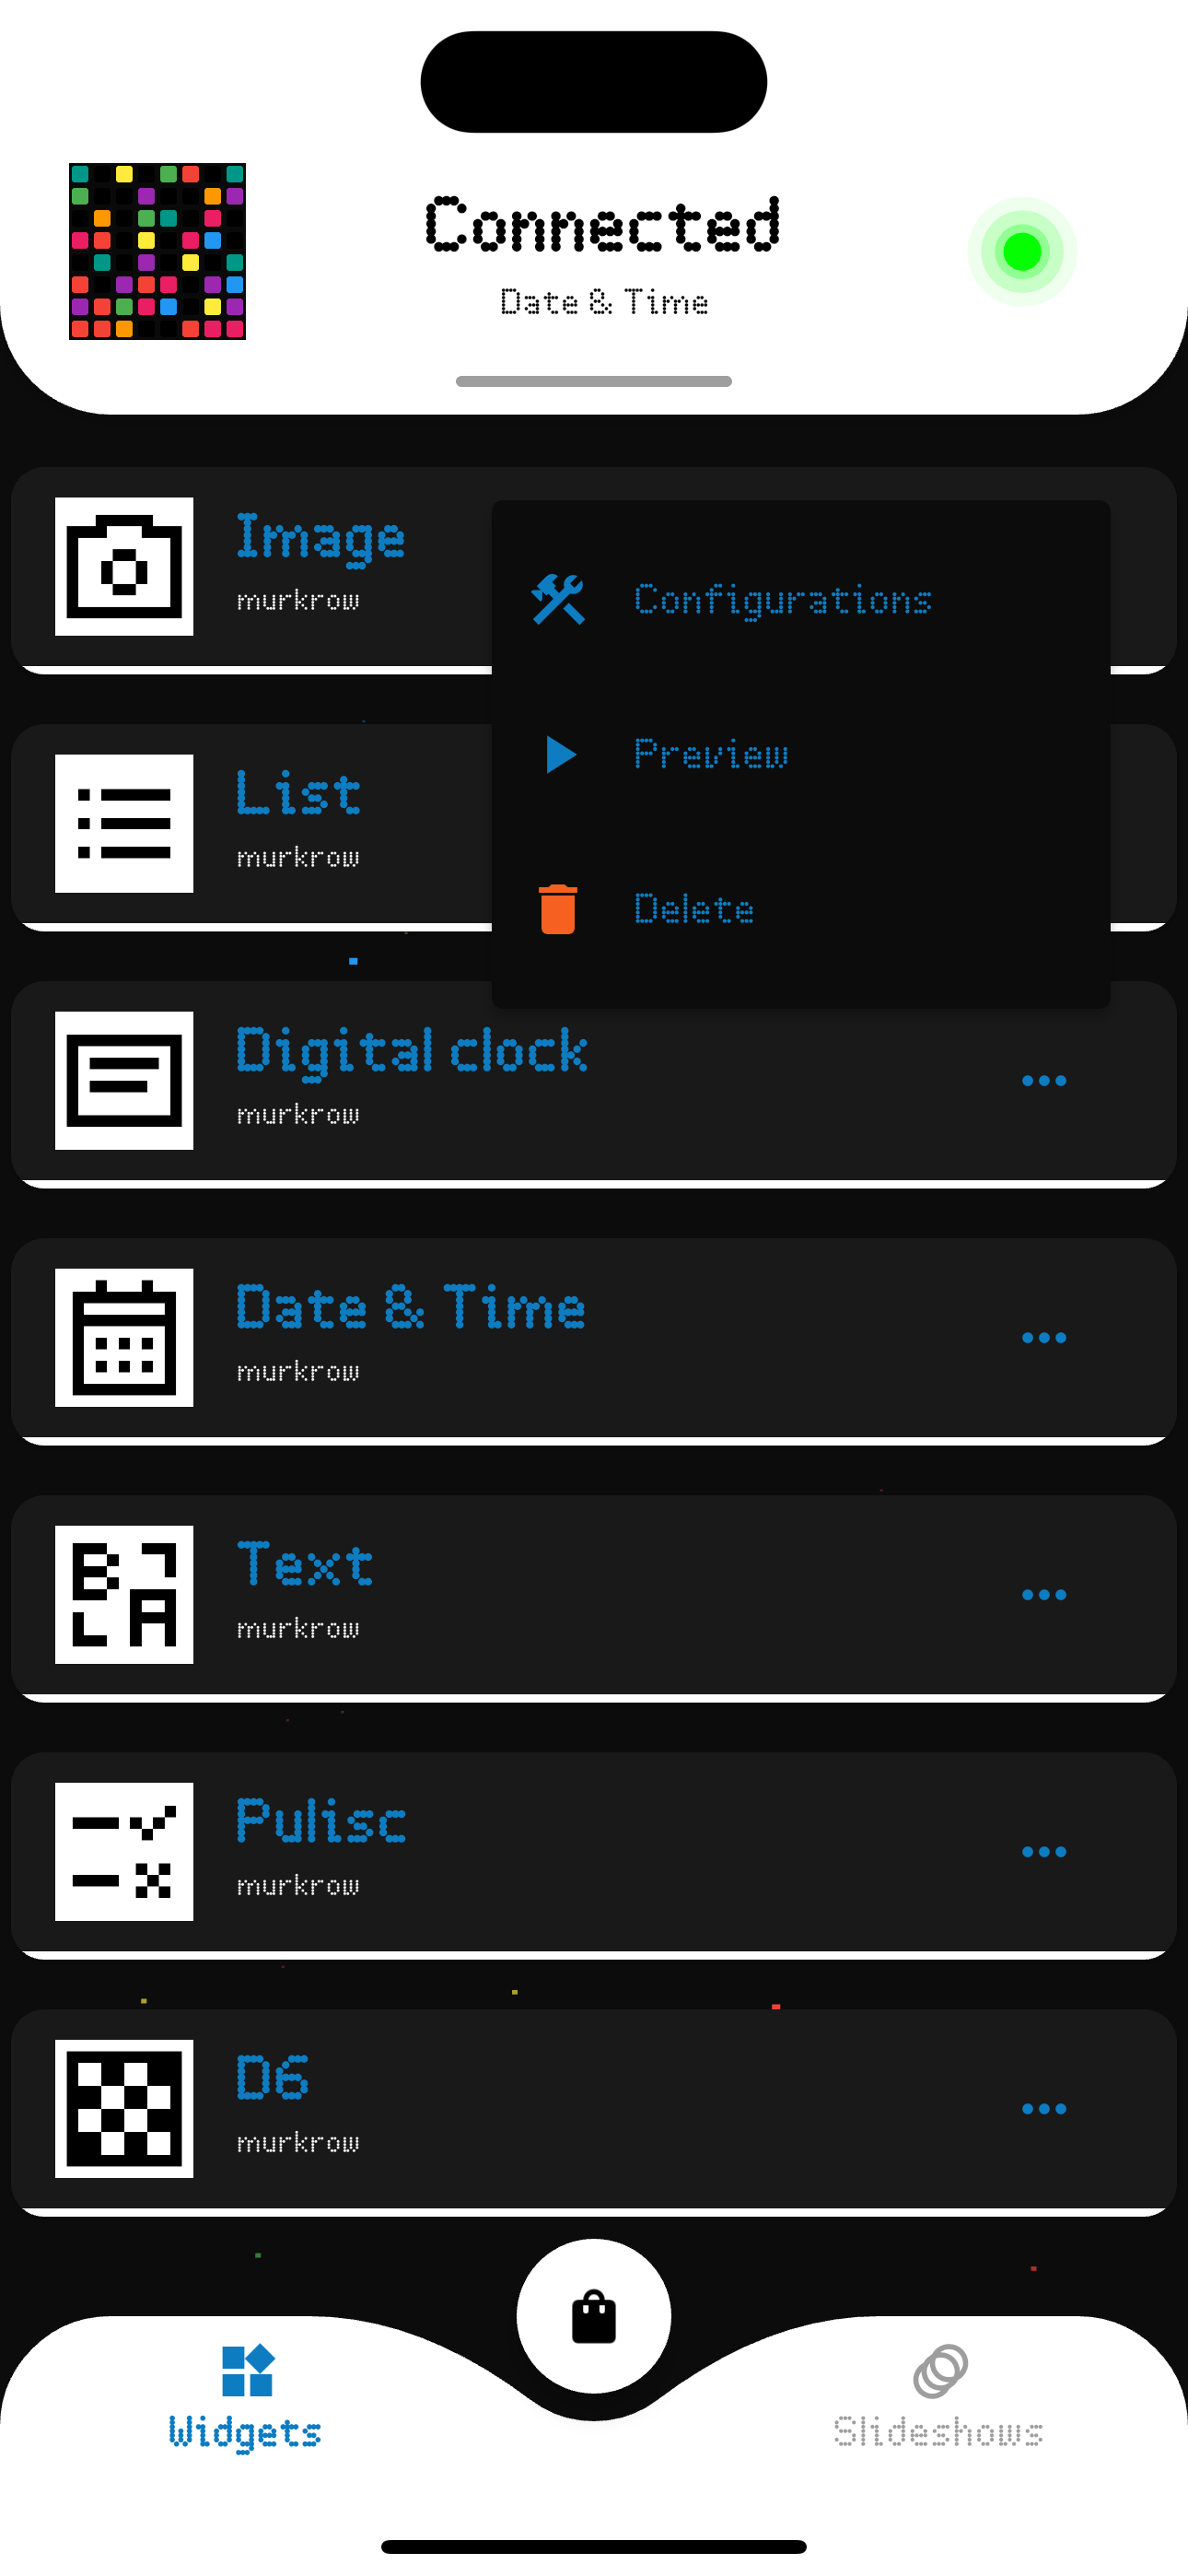
\includegraphics[width=\textwidth]{tesi/img/client_demo/installed_widgets/page.png}
        \caption*{Installed Widget Actions}
    \end{minipage}
    \begin{minipage}[b]{0.32\textwidth}
        \centering
        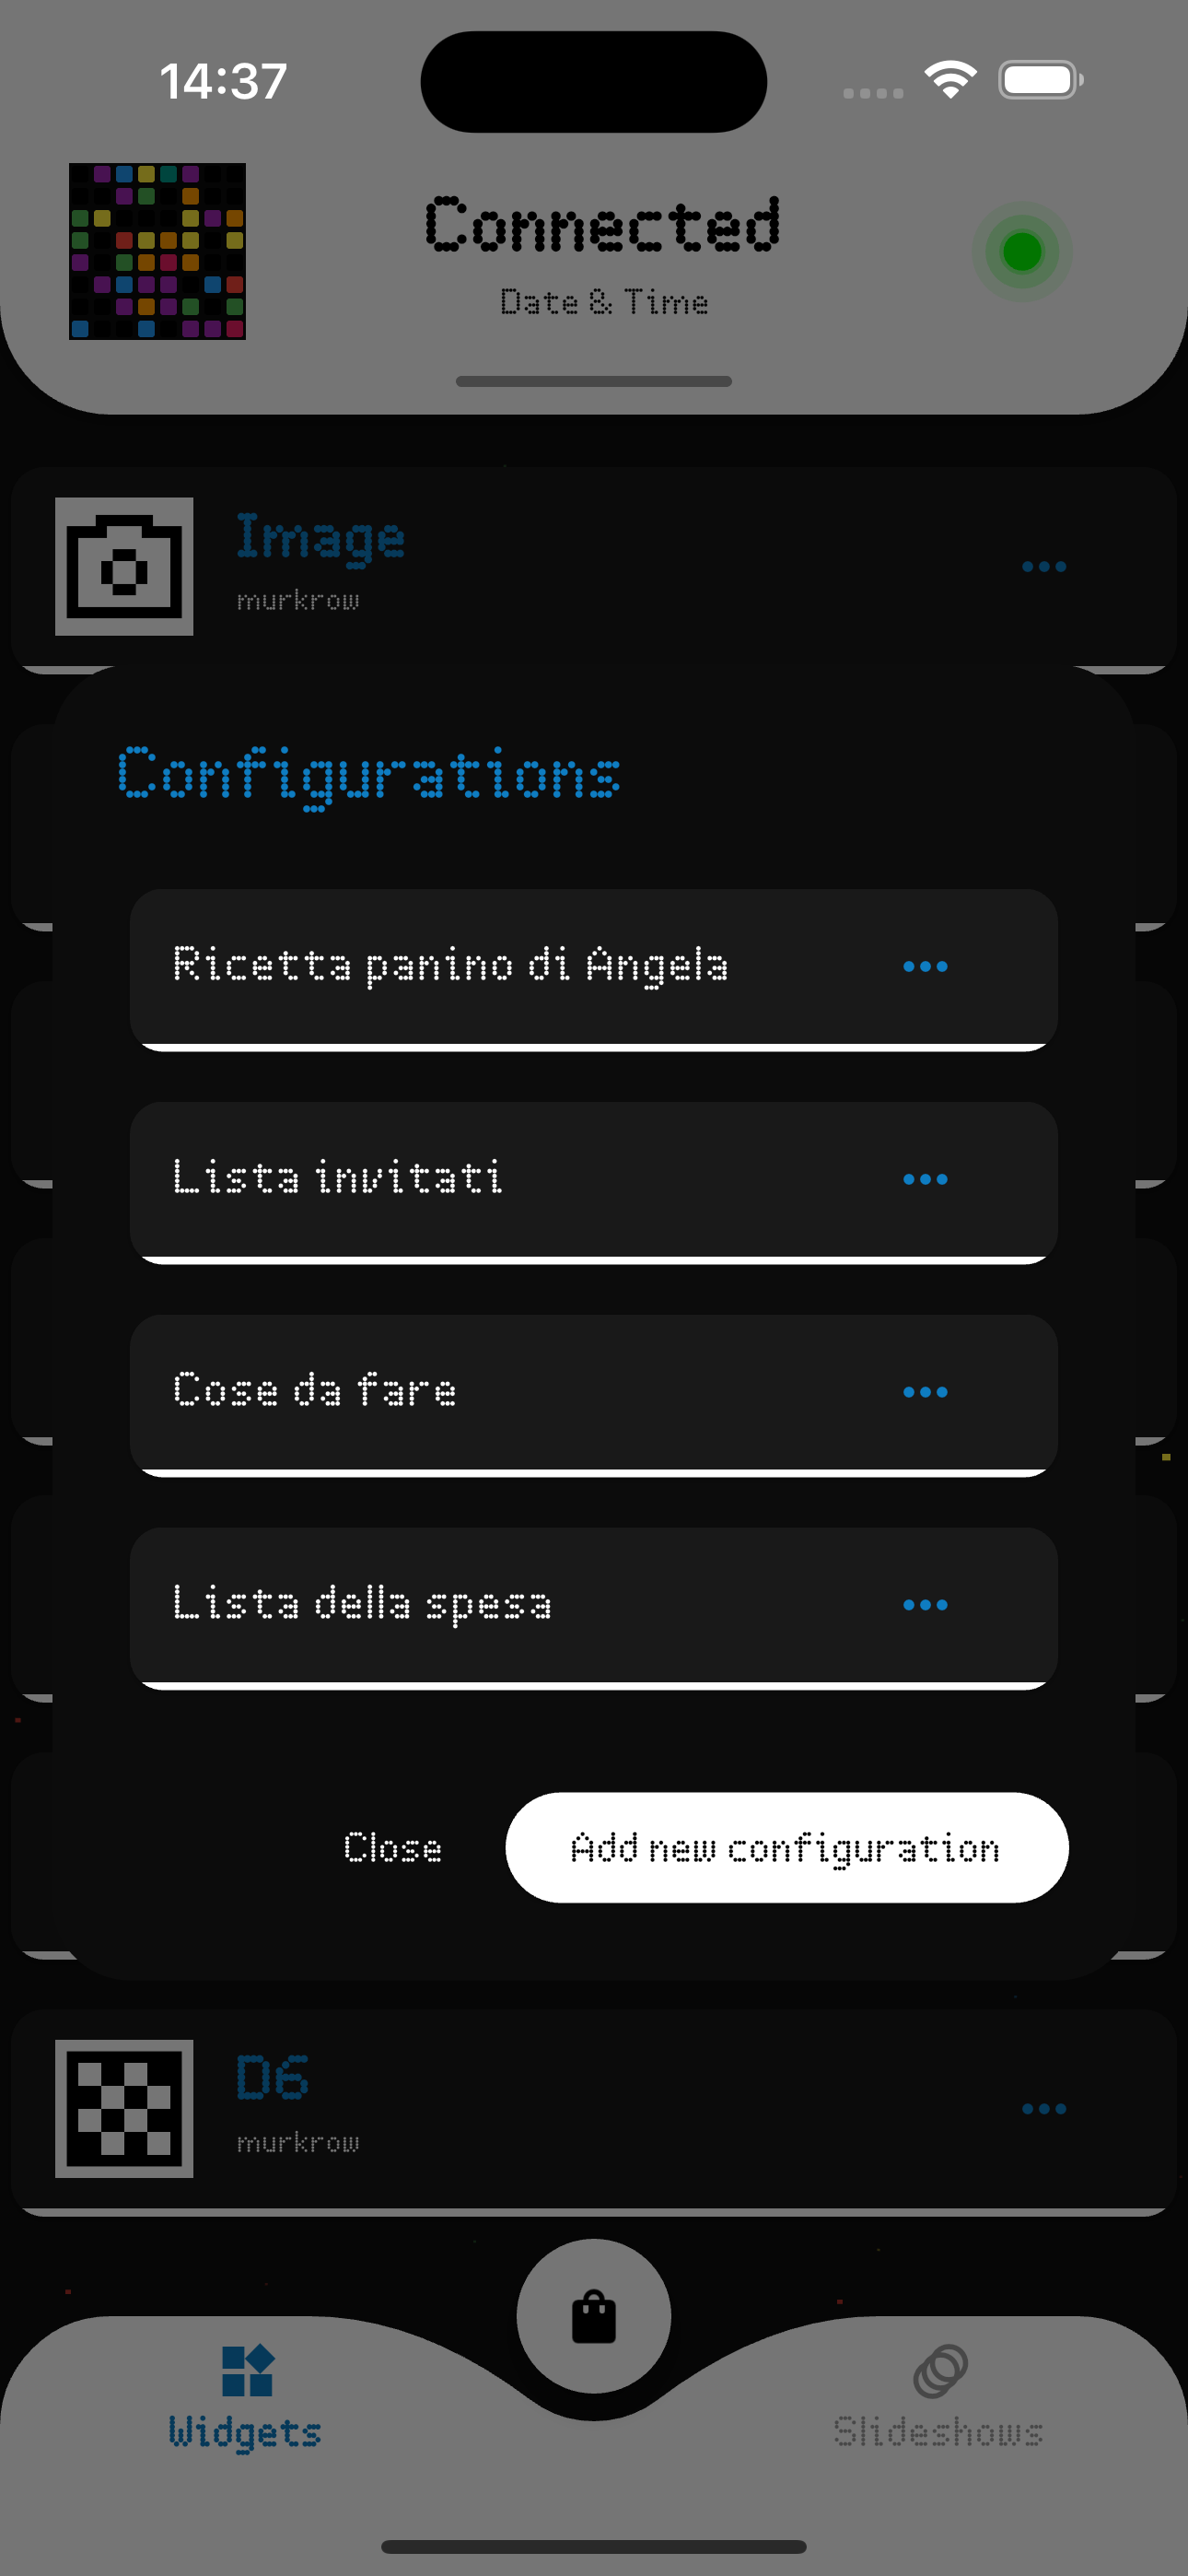
\includegraphics[width=\textwidth]{tesi/img/client_demo/installed_widgets/config_choice.png}
        \caption*{Configuration Selector}
    \end{minipage}
\end{figure}
\newpage
\subsection{Widget Store}
The widget store provides users with a space to discover new widgets. A main page lists all available widgets, each represented by a tile. By clicking on a tile, users can view more detailed information about the widget, including an image carousel, a rich markdown description, and details about the widget’s author and source code. Notably, all widgets in the store must be uploaded to a publicly accessible repository, ensuring that the ecosystem remains entirely open-source.

\begin{figure}[h]
    \centering
    \begin{minipage}[b]{0.32\textwidth}
        \centering
        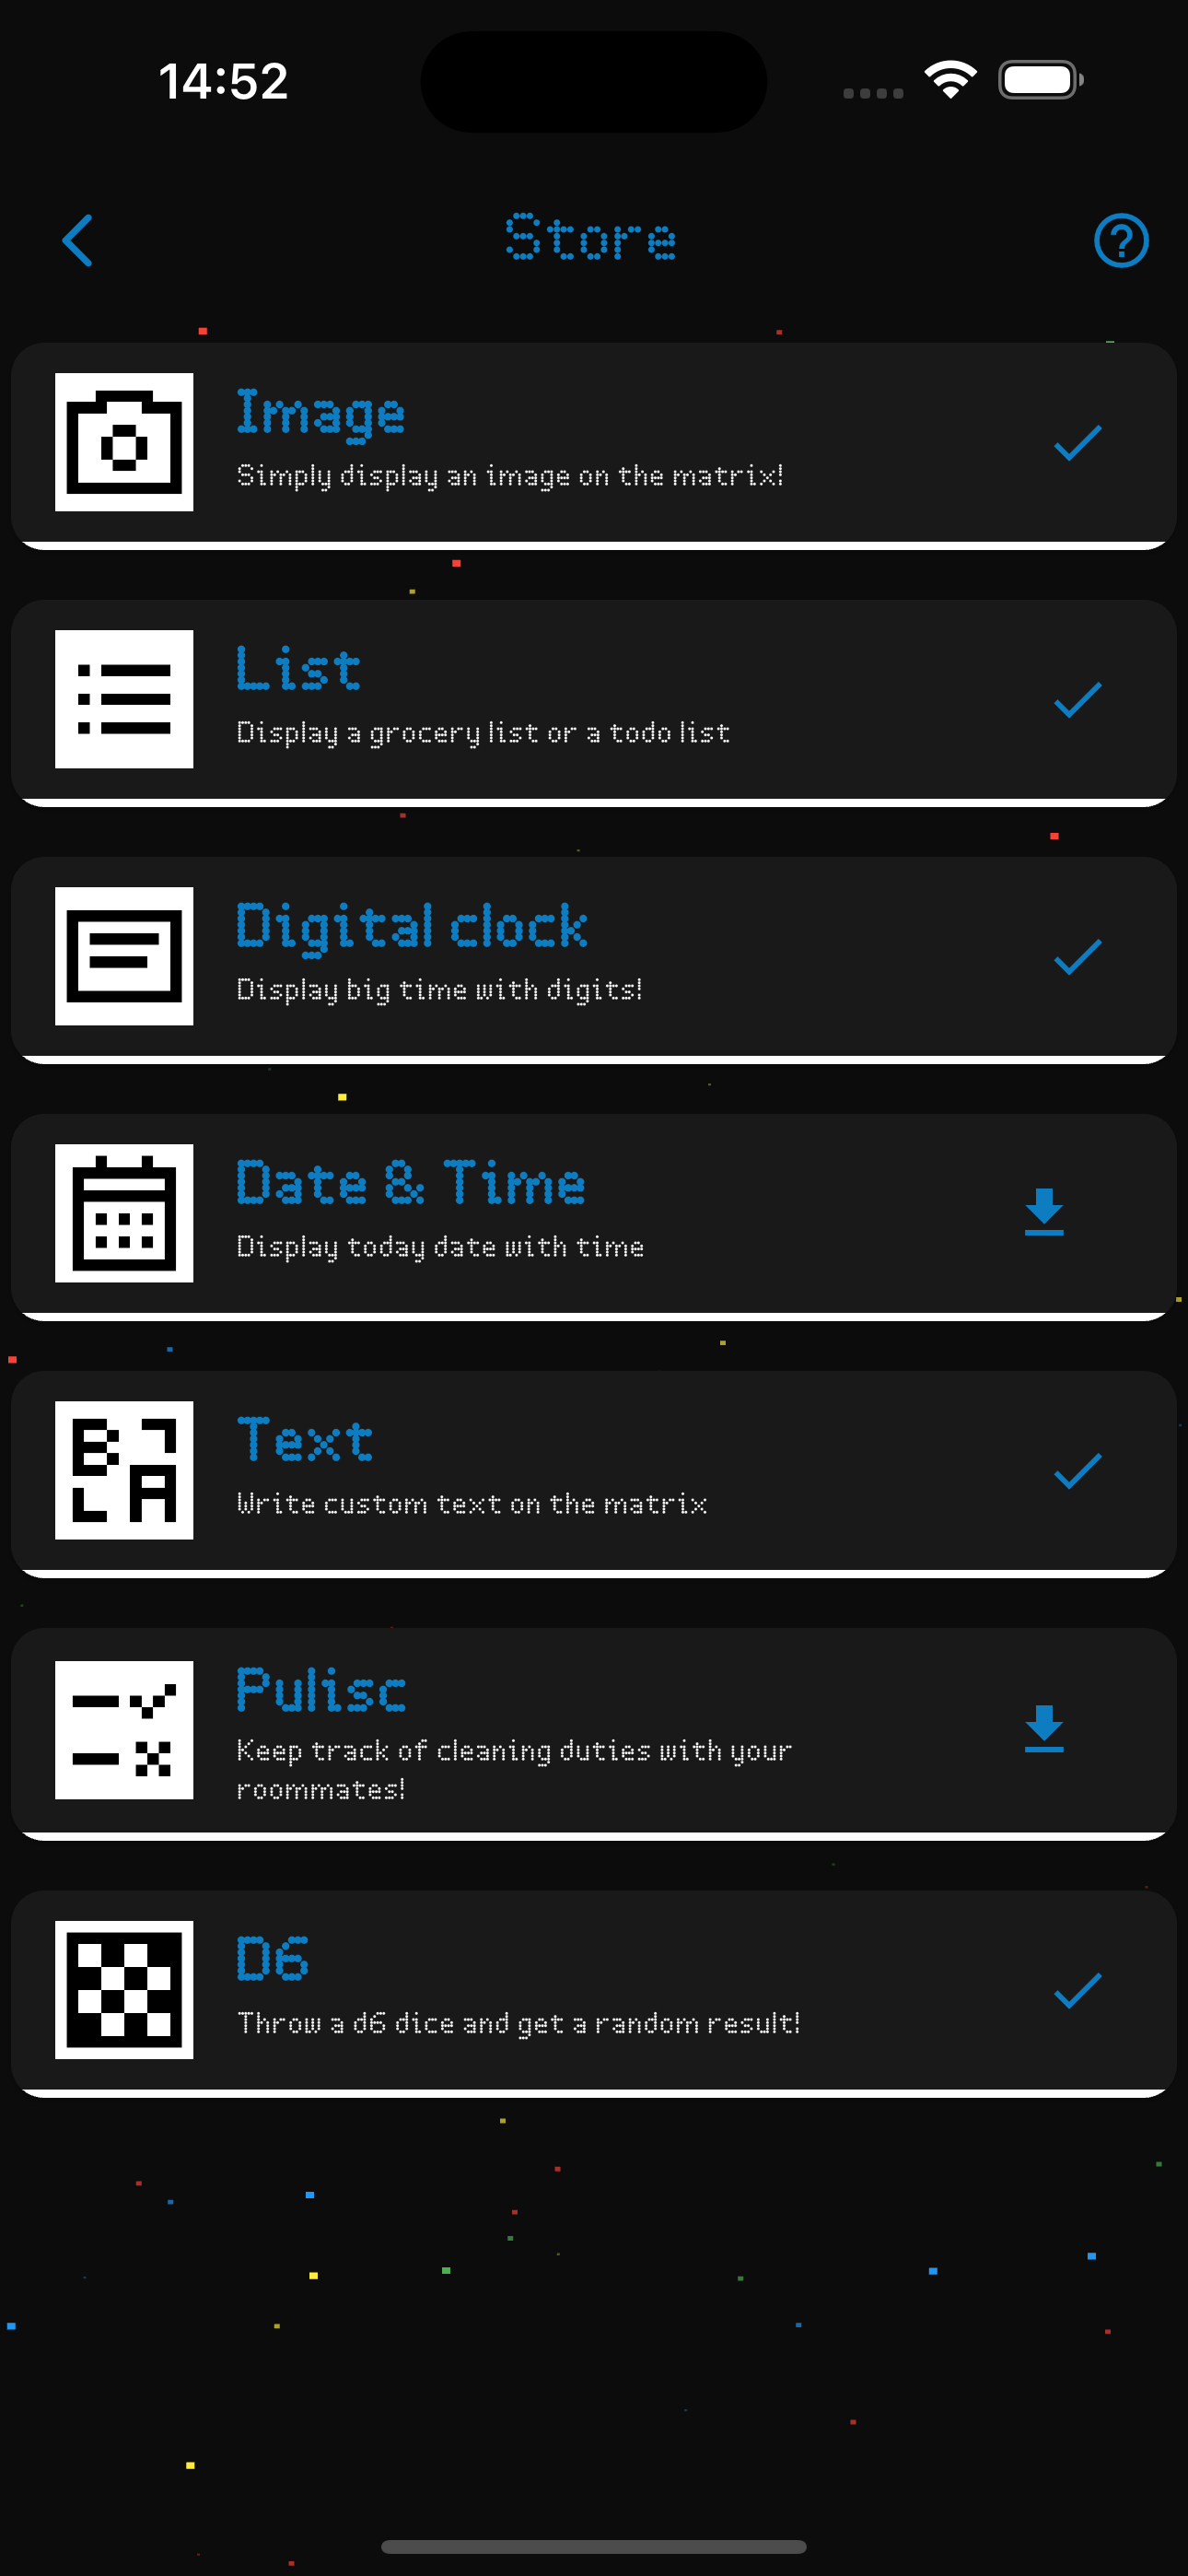
\includegraphics[width=\textwidth]{tesi/img/client_demo/store/page.png}
        \caption*{Store Overview}
    \end{minipage}
    \begin{minipage}[b]{0.32\textwidth}
        \centering
        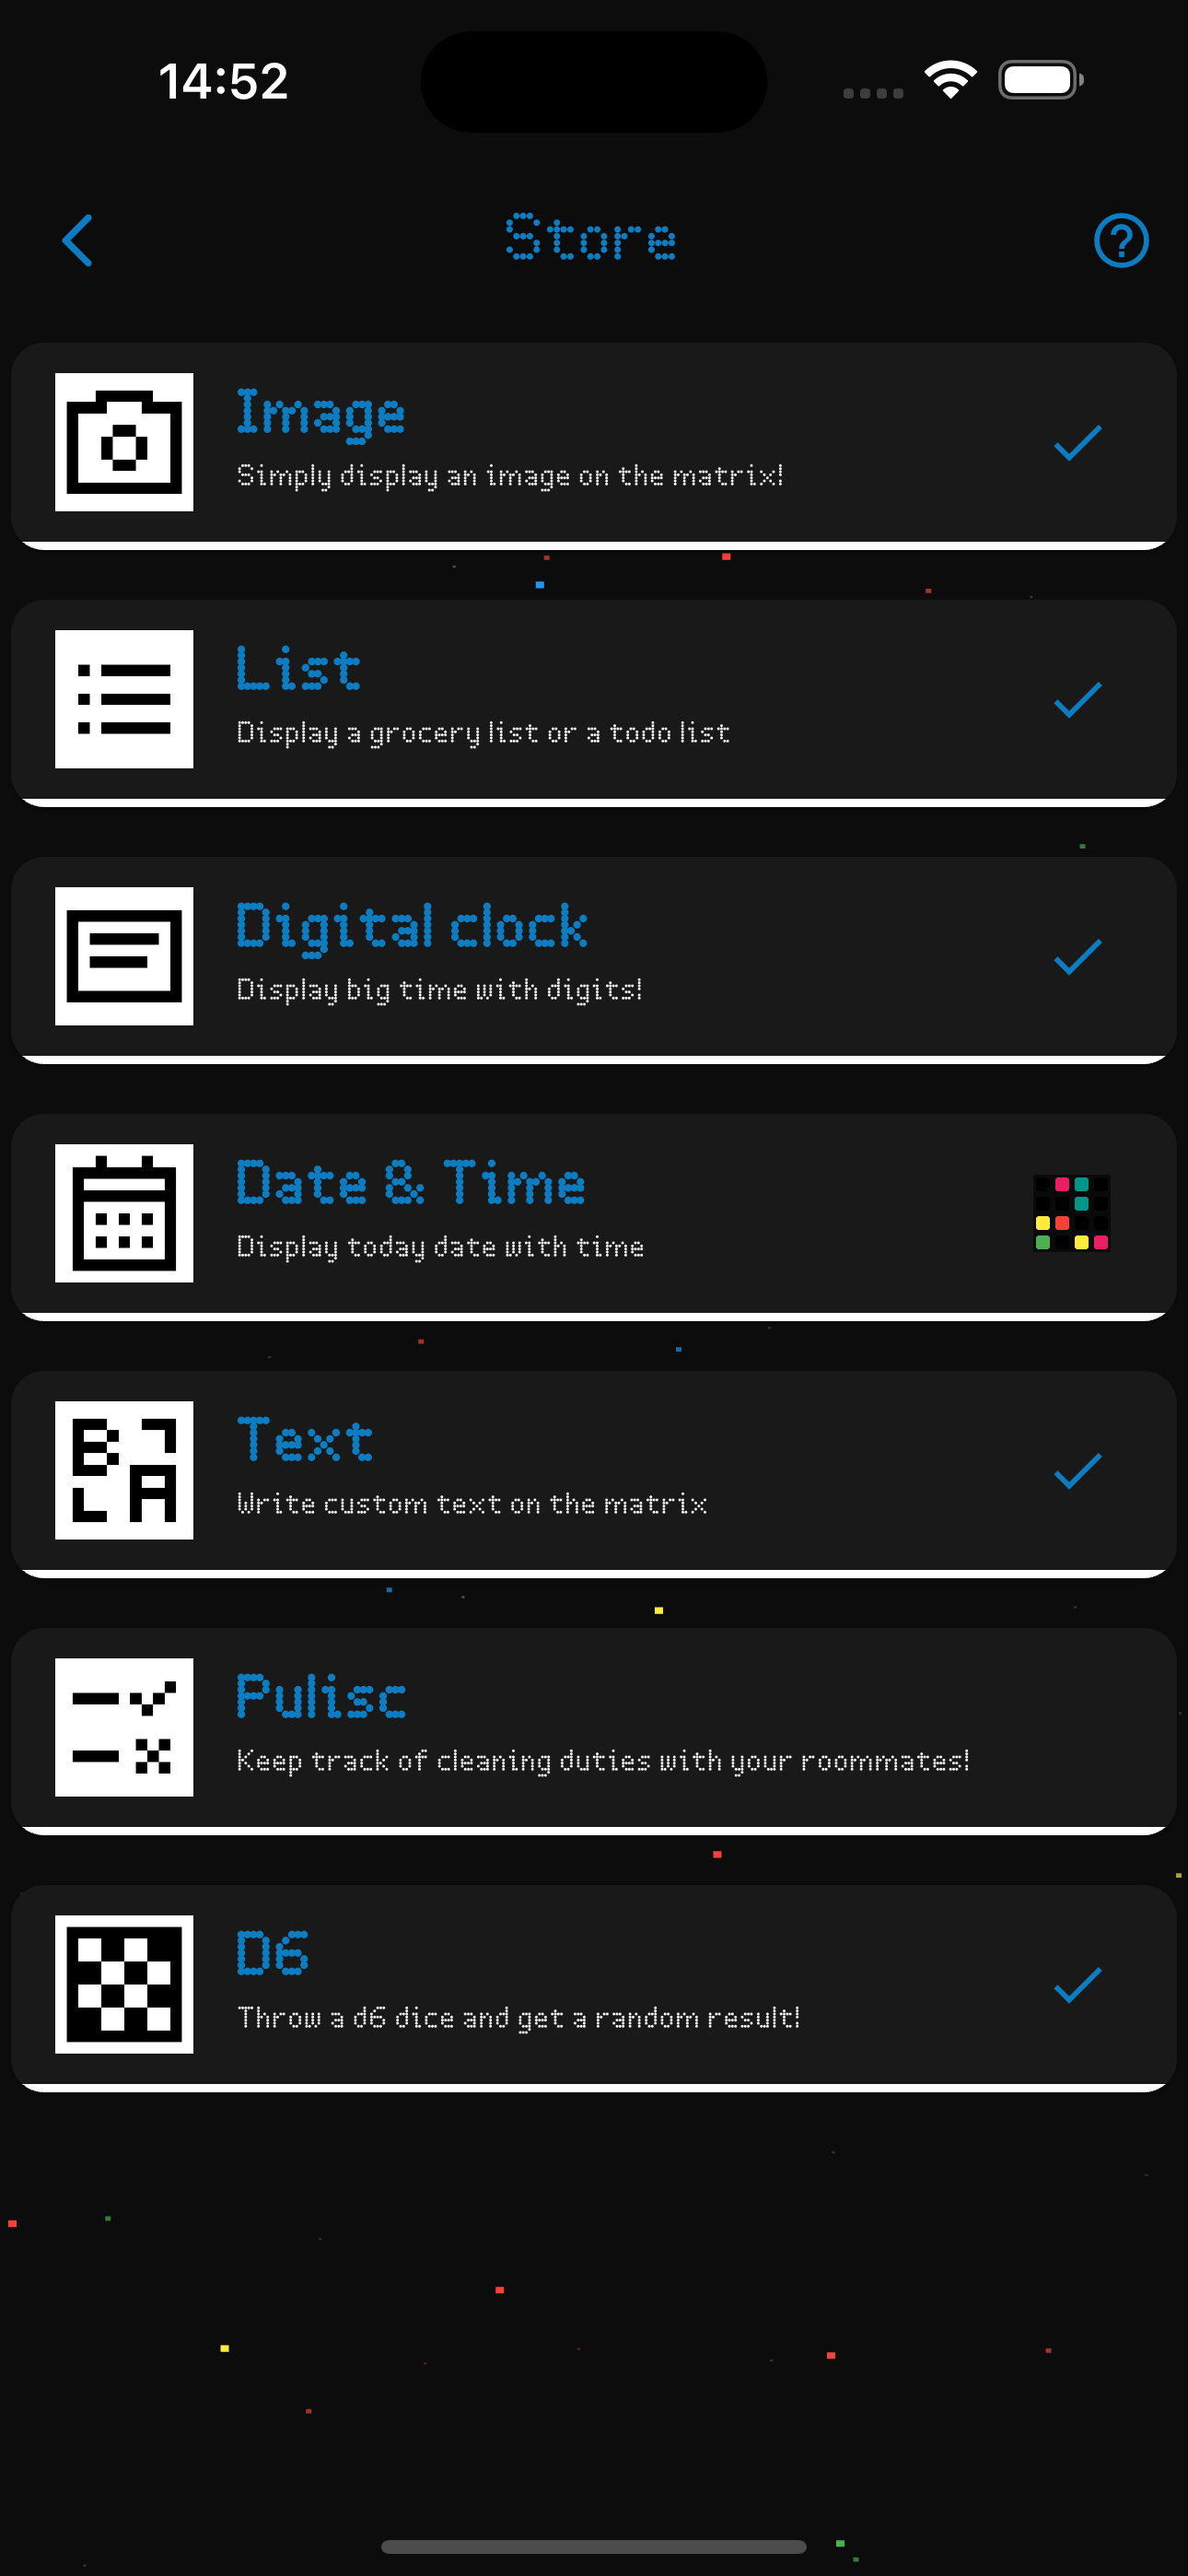
\includegraphics[width=\textwidth]{tesi/img/client_demo/store/widget_installing.png}
        \caption*{Installing a Widget}
    \end{minipage}
    \begin{minipage}[b]{0.32\textwidth}
        \centering
        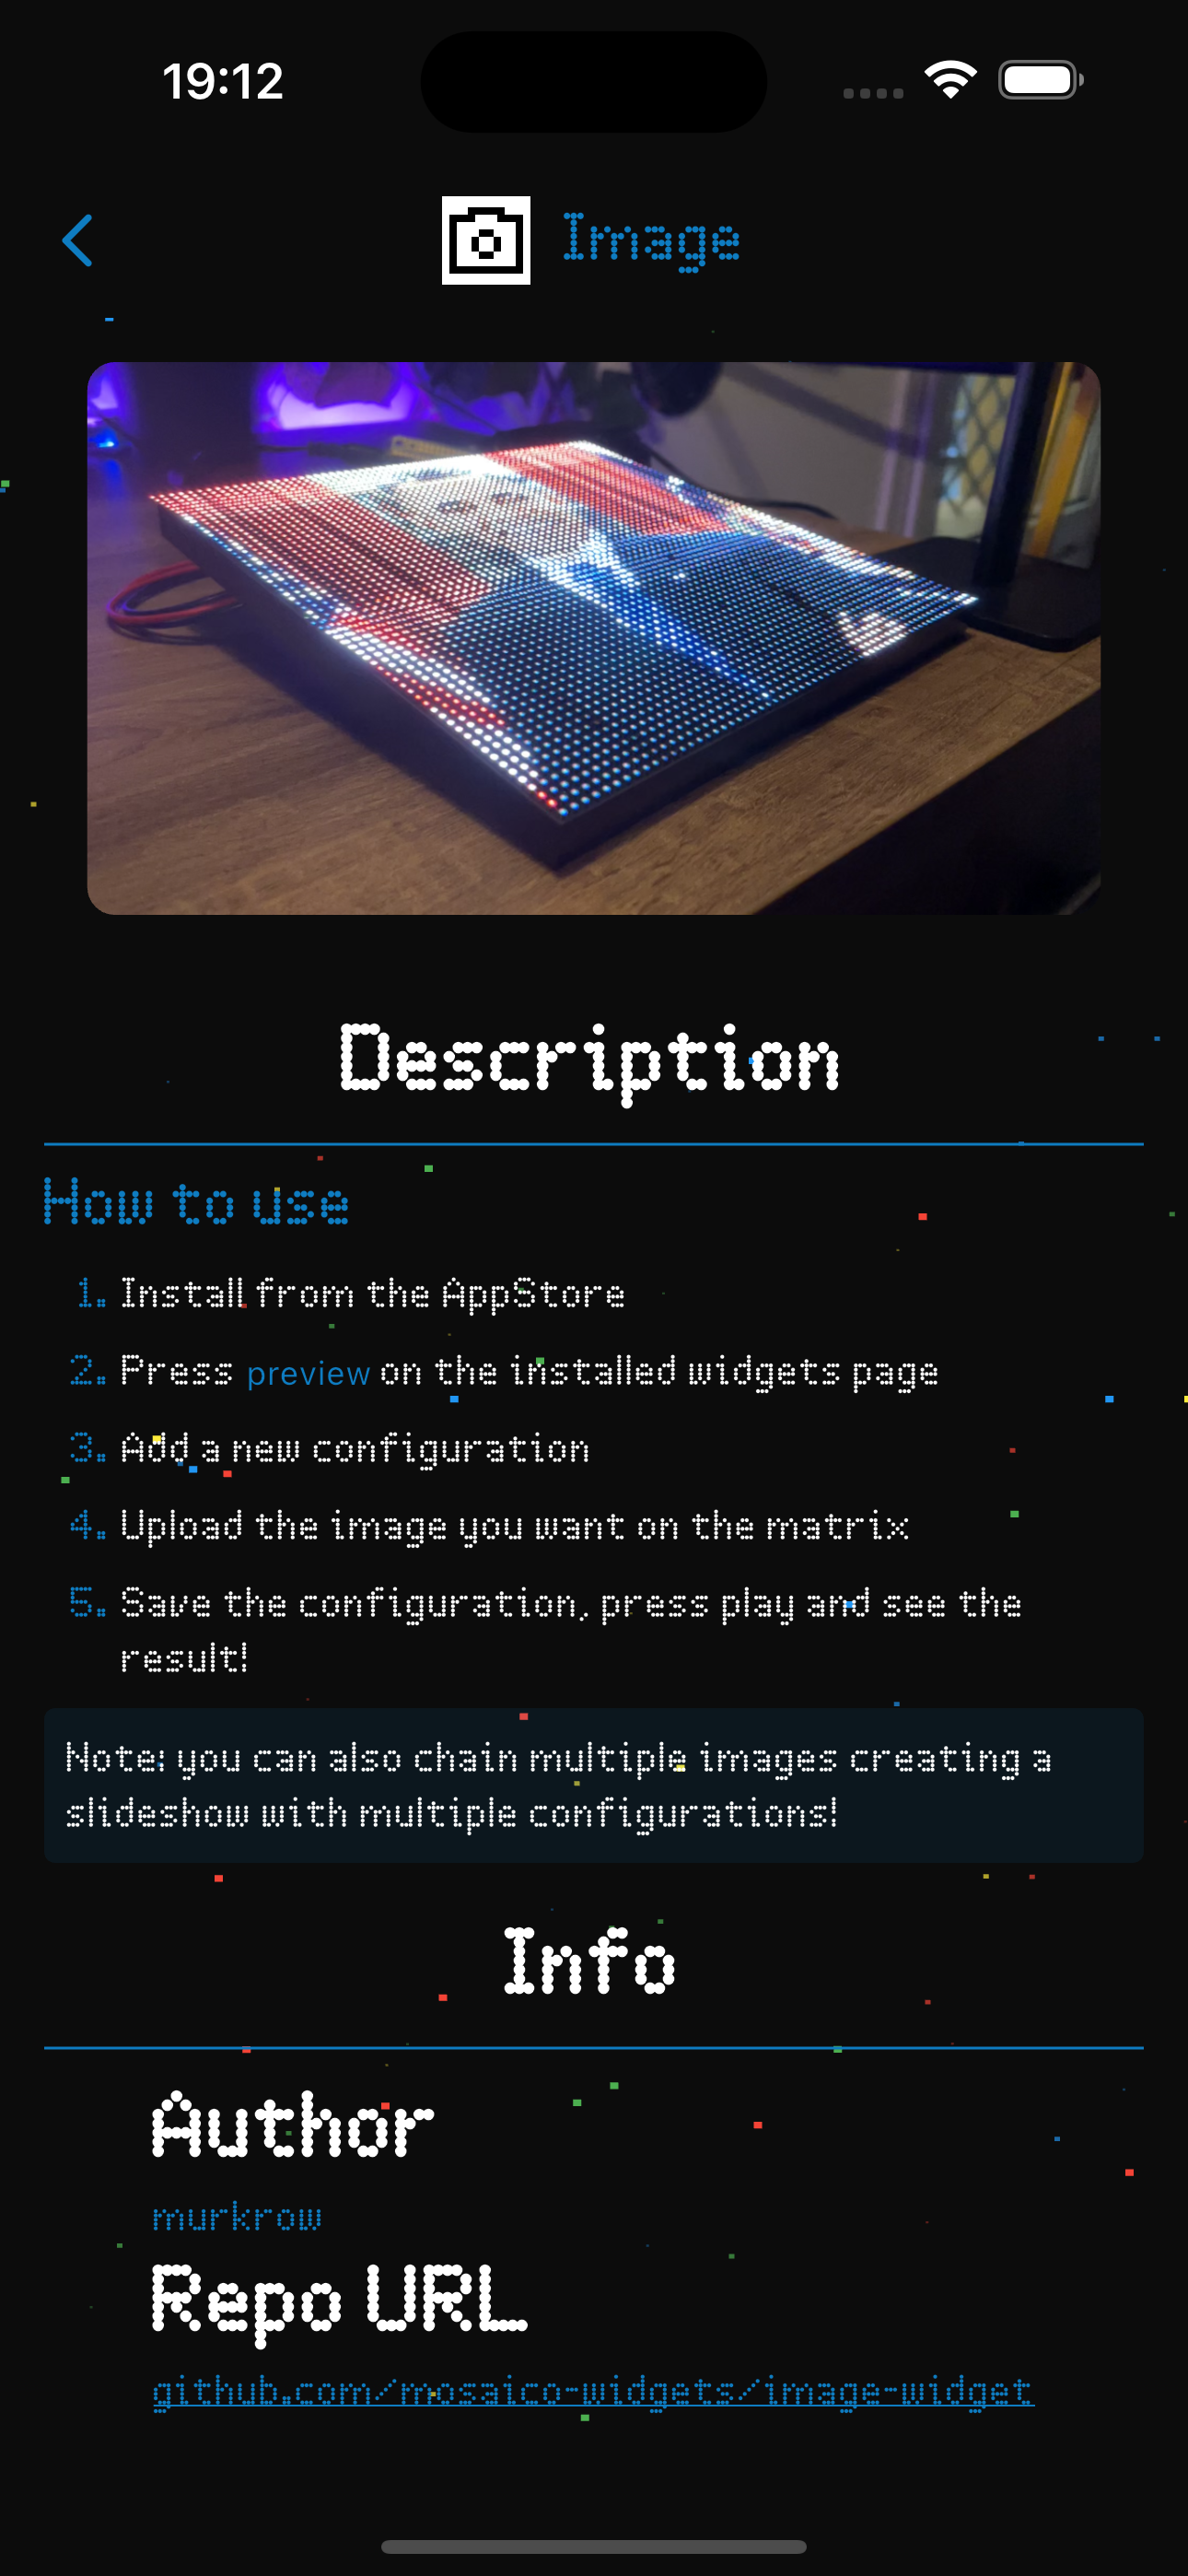
\includegraphics[width=\textwidth]{tesi/img/client_demo/store.png}
        \caption*{Widget Details}
    \end{minipage}
\end{figure}

\subsection{Slideshows}
Slideshows are sequences of widgets displayed consecutively on the matrix. This feature is particularly useful when users prefer to cycle through multiple widgets rather than display a single one continuously.

Creating a new slideshow is intuitive. Users are presented with cards containing two fields: a widget selector and a duration field where they can input the display time in seconds. If the selected widget is configurable, a third field will appear, allowing users to select a specific configuration for that item.

A floating action button in the bottom-right corner expands to provide three actions:
\begin{itemize}
    \item \textbf{Plus Icon}: Adds a new slideshow item card.
    \item \textbf{Save Icon}: Saves the current slideshow or creates a new one.
    \item \textbf{Play Icon}: Saves and immediately plays the current slideshow on the matrix.
\end{itemize}

\begin{figure}[h]
    \centering
    \begin{minipage}[b]{0.32\textwidth}
        \centering
        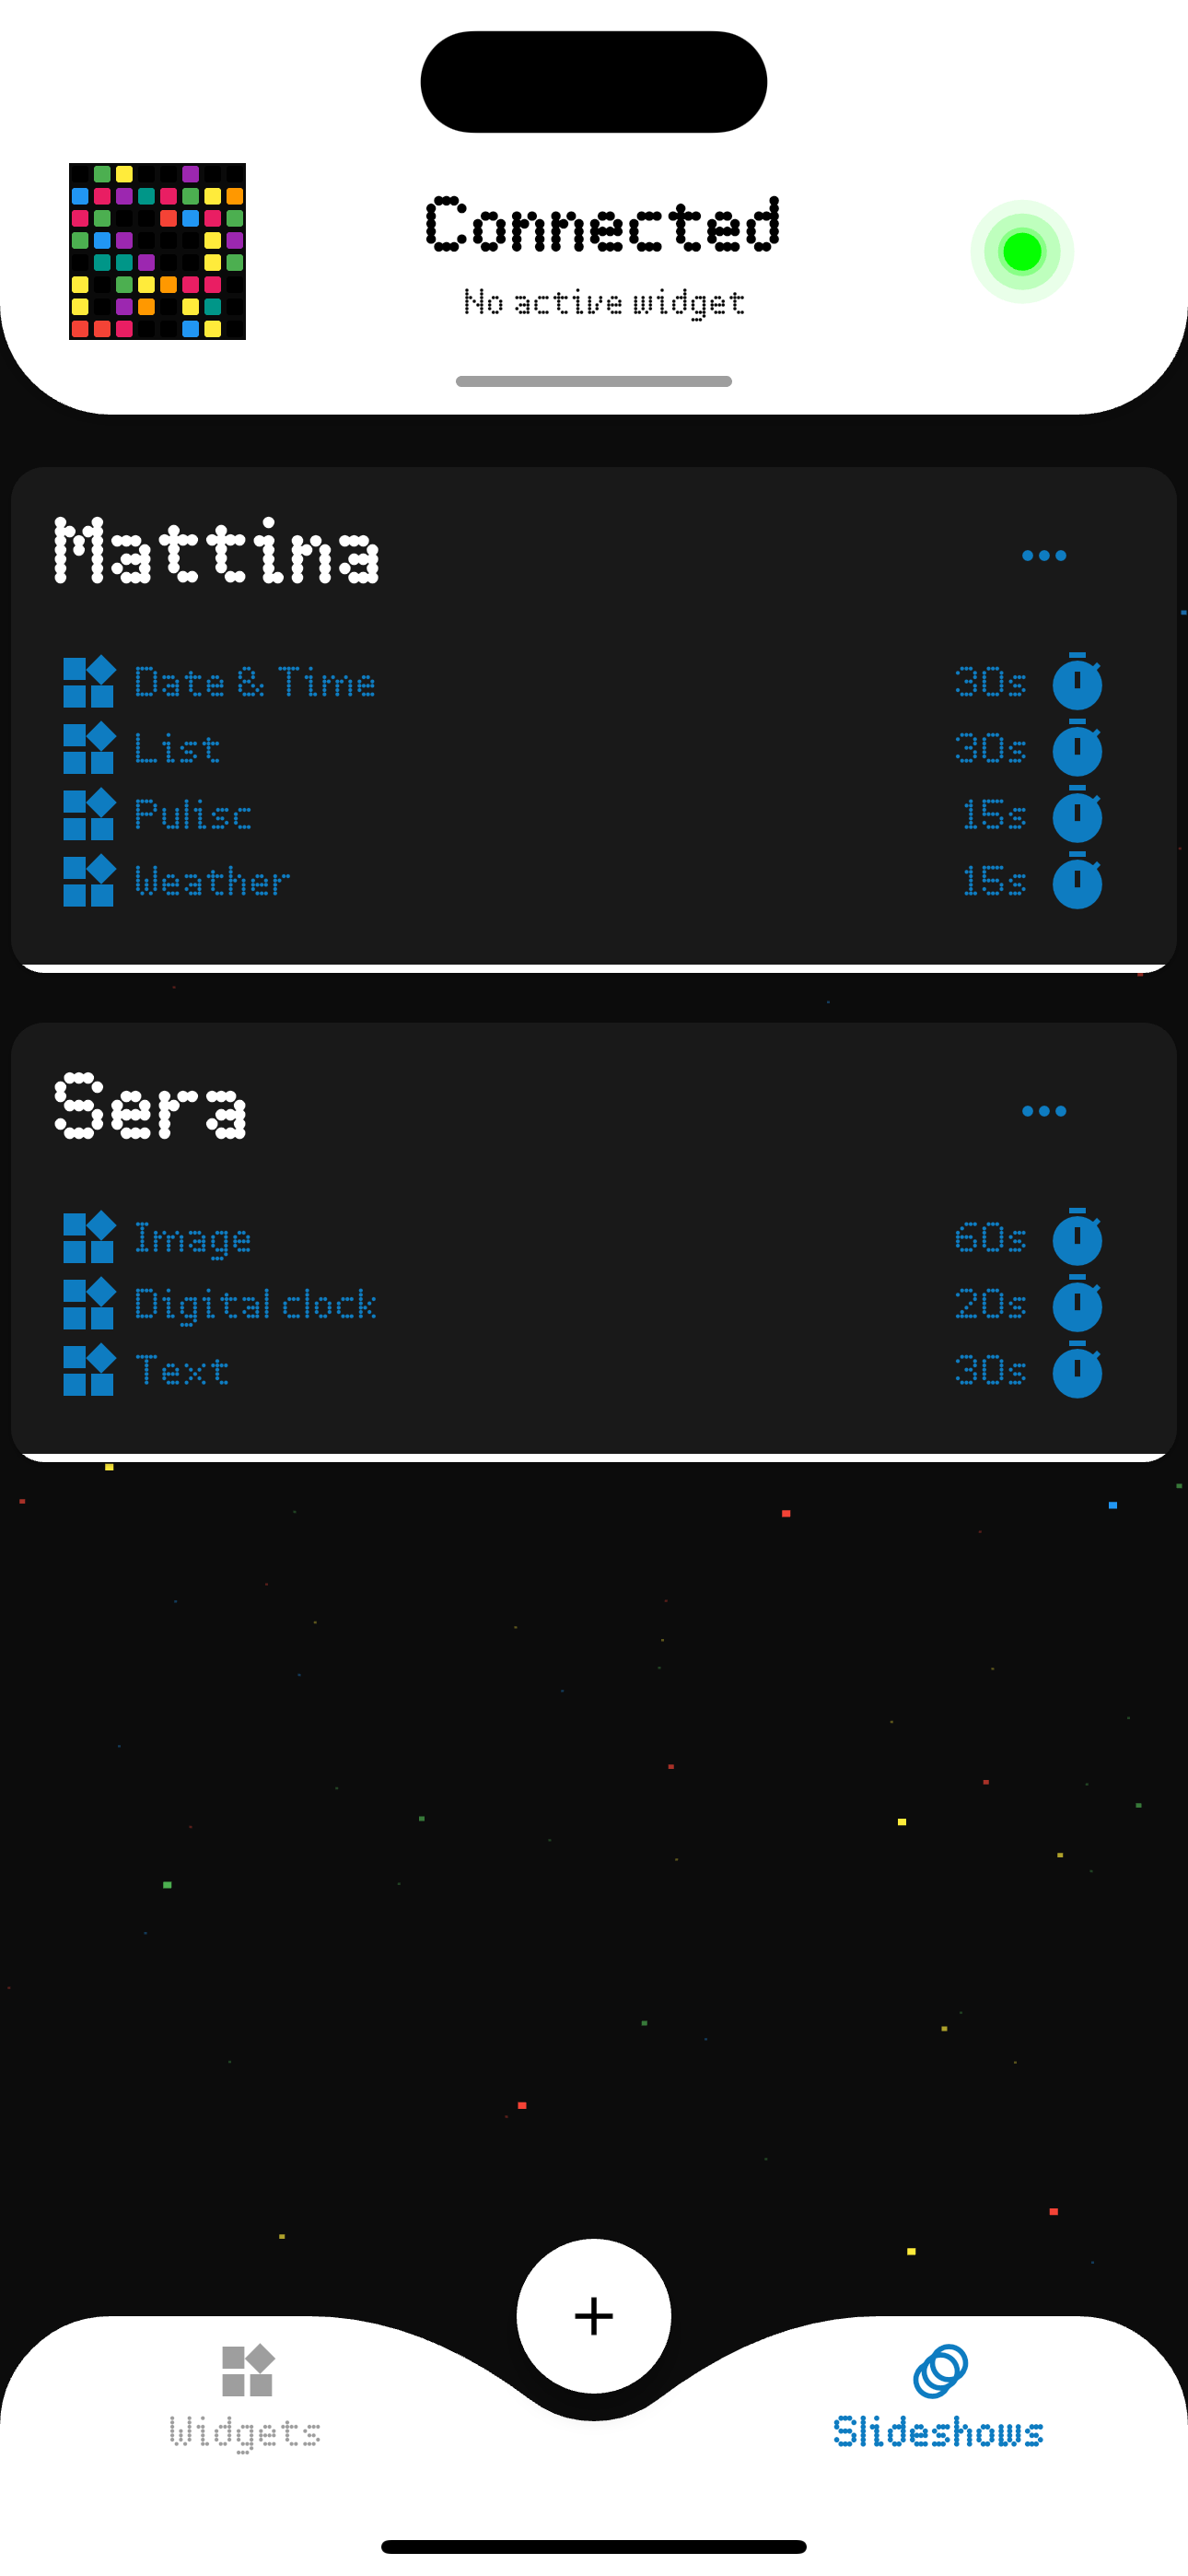
\includegraphics[width=\textwidth]{tesi/img/client_demo/slideshows/page.png}
        \caption*{Slideshows Page}
    \end{minipage}
    \begin{minipage}[b]{0.32\textwidth}
        \centering
        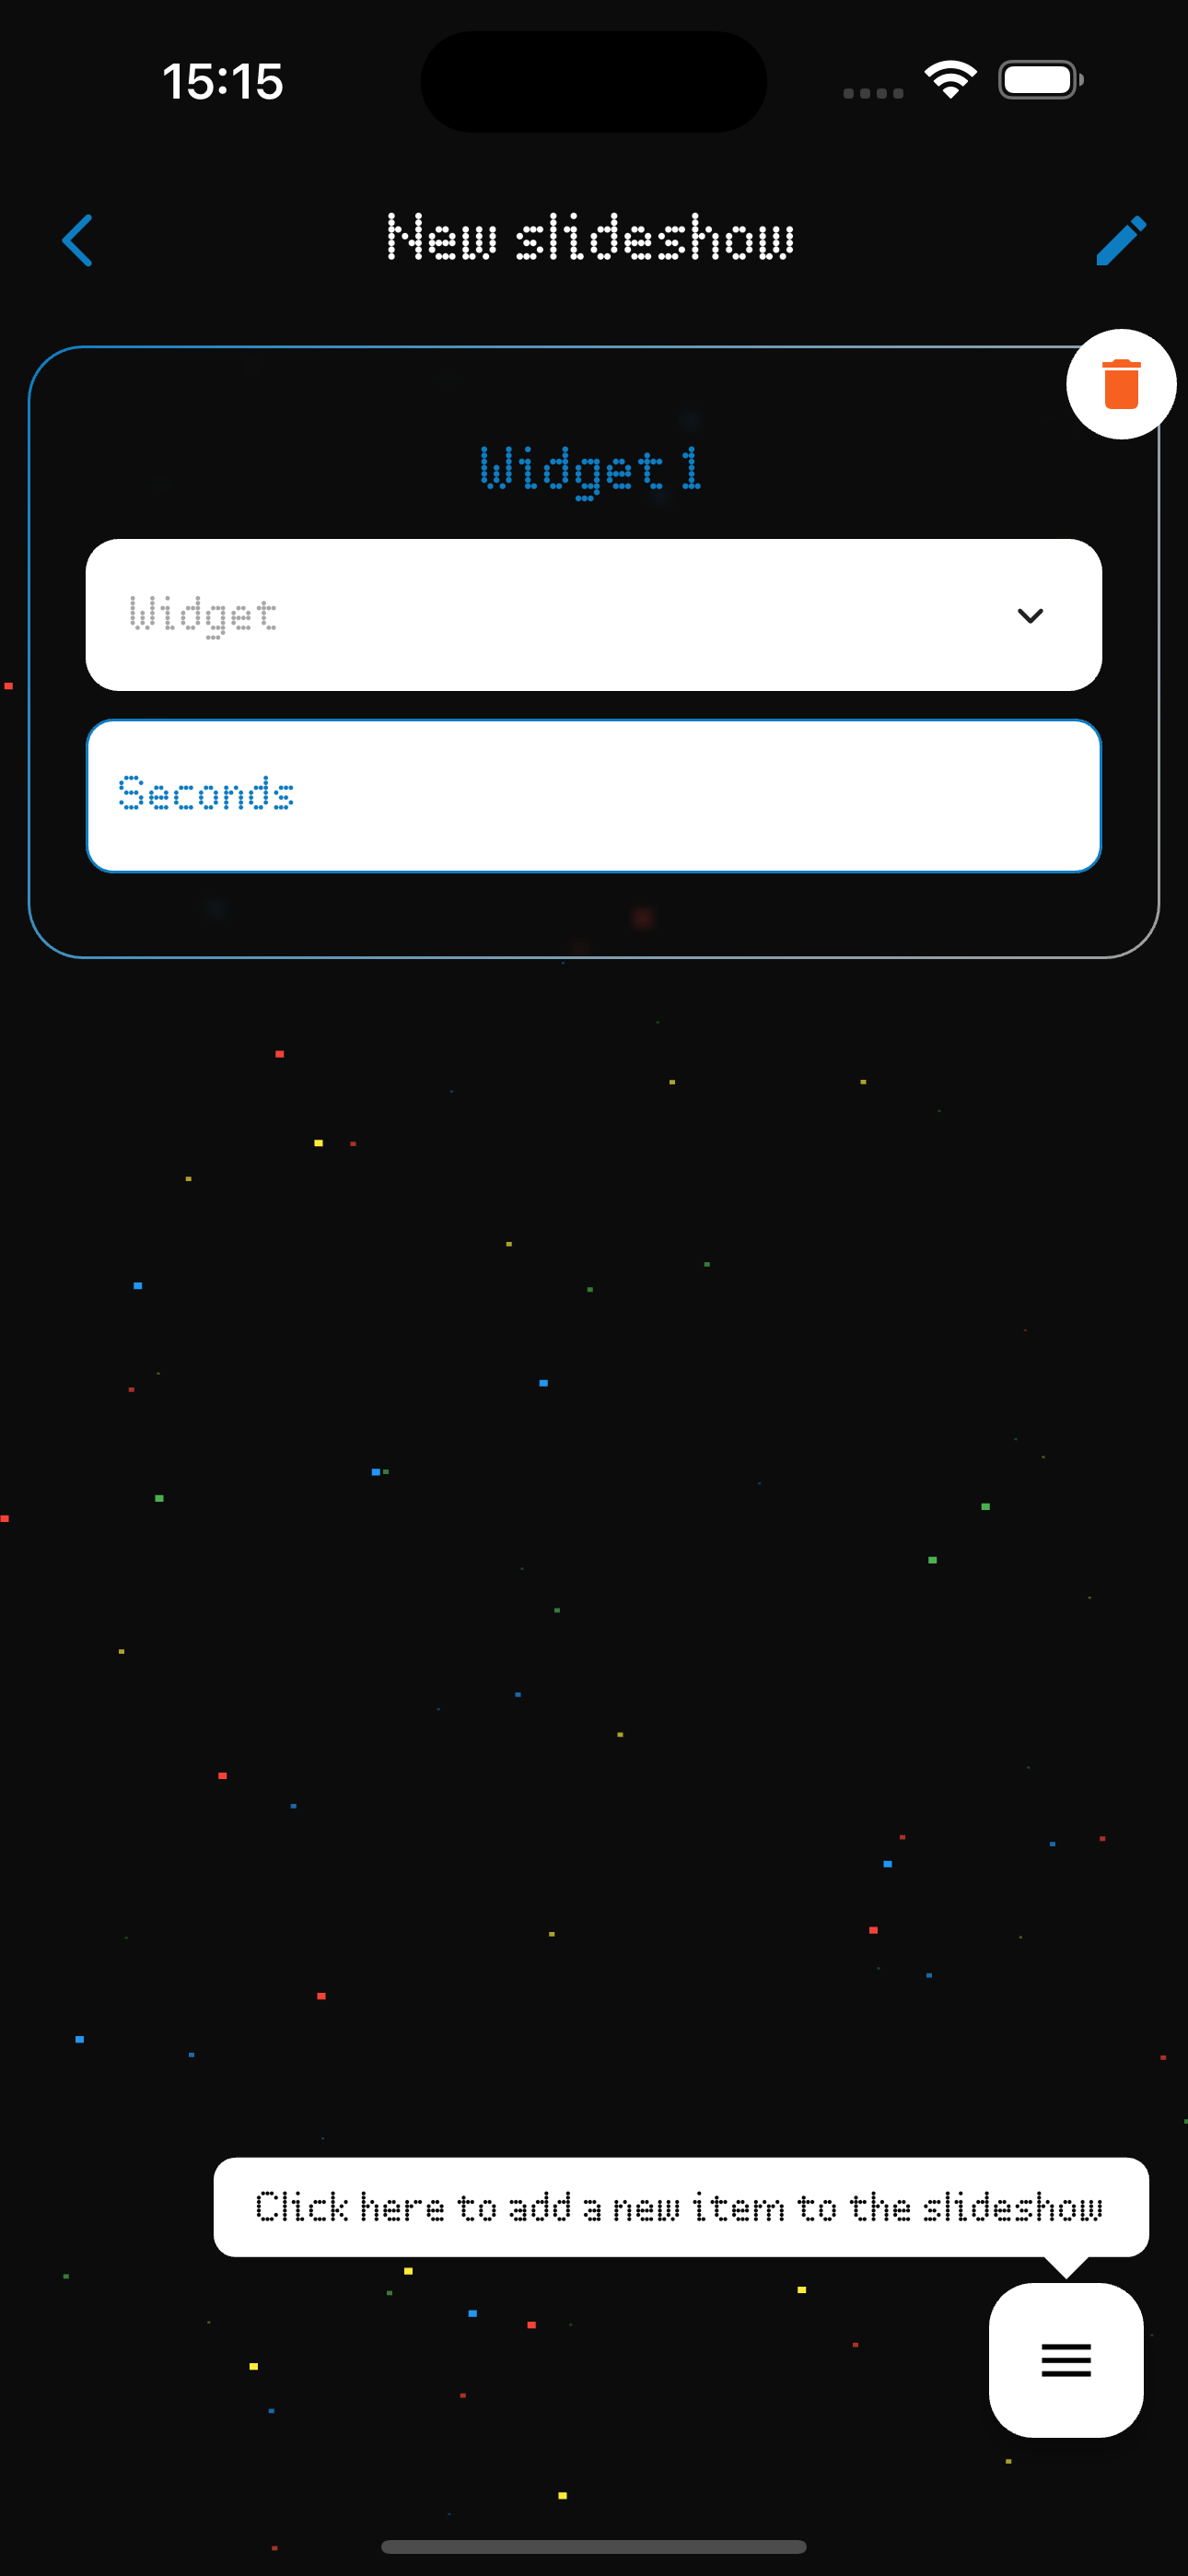
\includegraphics[width=\textwidth]{tesi/img/client_demo/slideshows/new.png}
        \caption*{Create a New Slideshow}
    \end{minipage}
    \begin{minipage}[b]{0.32\textwidth}
        \centering
        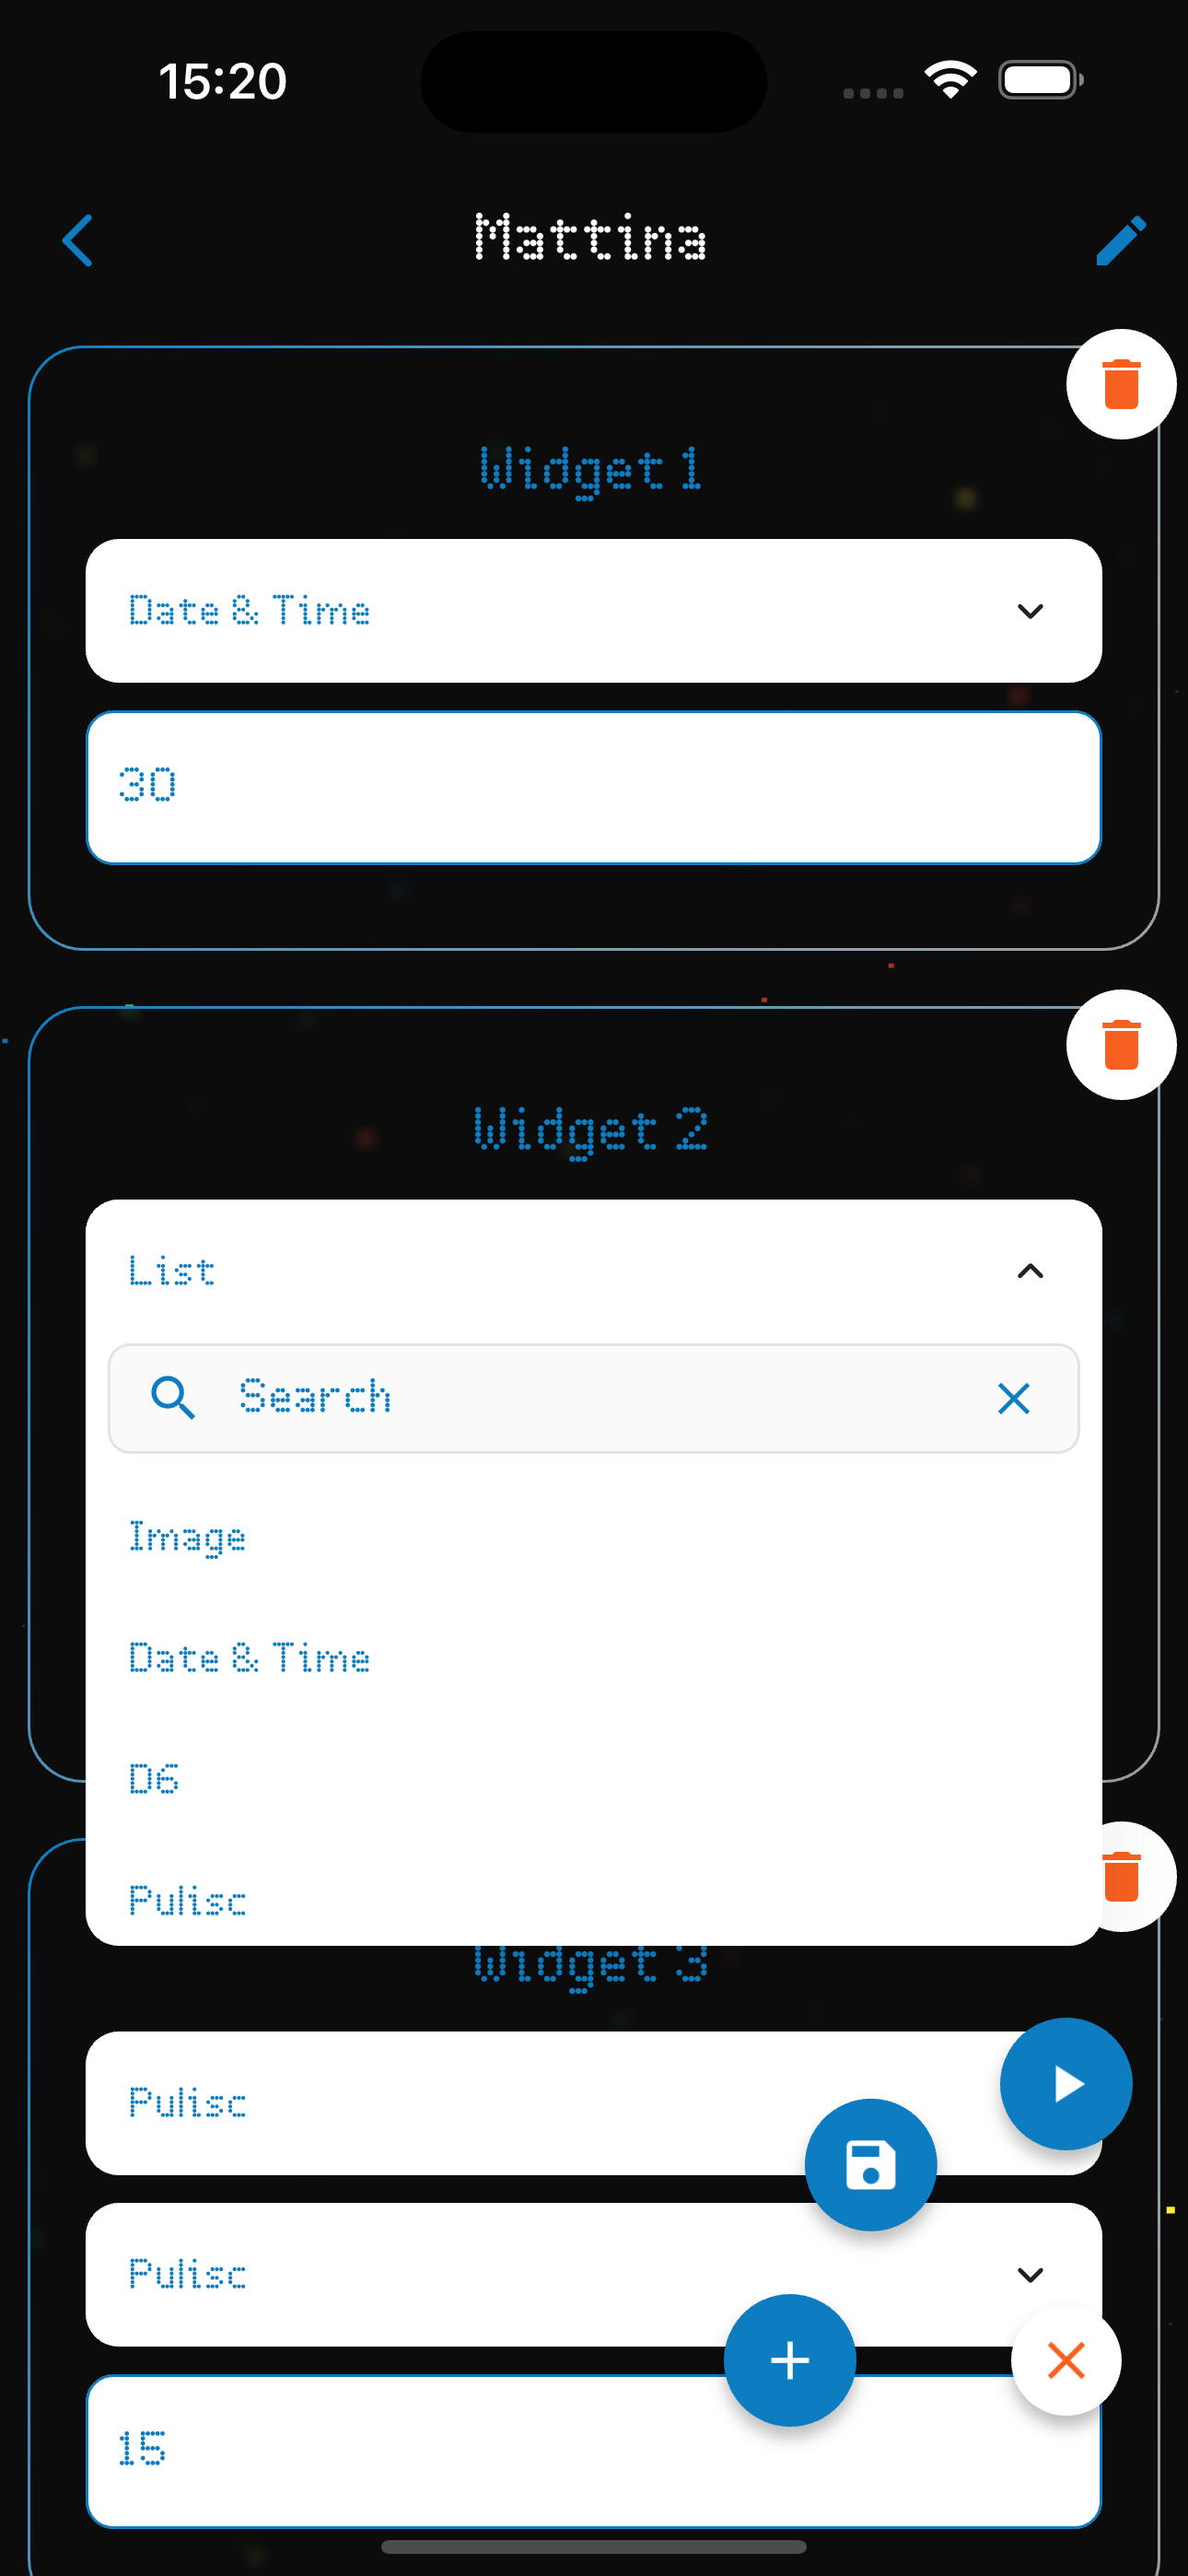
\includegraphics[width=\textwidth]{tesi/img/client_demo/slideshows/edit.png}
        \caption*{Edit an Existing Slideshow}
    \end{minipage}
\end{figure}